%"runningheads" enables:
%  - page number on page 2 onwards
%  - title/authors on even/odd pages
%This is good for other readers to enable proper archiving among other papers and pointing to content.

%Even though `american`, `english` and `USenglish` are synonyms for babel package (according to https://tex.stackexchange.com/questions/12775/babel-english-american-usenglish), the llncs document class is prepared to avoid the overriding of certain names (such as "Abstract." -> "Abstract" or "Fig." -> "Figure") when using `english`, but not when using the other 2.
\documentclass[runningheads,a4paper]{llncs}
\usepackage[english]{babel}

%better font, similar to the default springer font
%cfr-lm is preferred over lmodern. Reasoning at http://tex.stackexchange.com/a/247543/9075
\usepackage[%
rm={oldstyle=false,proportional=true},%
sf={oldstyle=false,proportional=true},%
tt={oldstyle=false,proportional=true,variable=true},%
qt=false%
]{cfr-lm}
%
%if more space is needed, exchange cfr-lm by mathptmx
%\usepackage{mathptmx}

\usepackage{graphicx}

%extended enumerate, such as \begin{compactenum}
\usepackage{paralist}

%put figures inside a text
%\usepackage{picins}
%use
%\piccaptioninside
%\piccaption{...}
%\parpic[r]{\includegraphics ...}
%Text...

%Sorts the citations in the brackets
%\usepackage{cite}

\usepackage[T1]{fontenc}

%for demonstration purposes only
\usepackage[math]{blindtext}

%for easy quotations: \enquote{text}
\usepackage{csquotes}

%enable margin kerning
\usepackage{microtype}

%tweak \url{...}
\usepackage{url}
%nicer // - solution by http://tex.stackexchange.com/a/98470/9075
\makeatletter
\def\Url@twoslashes{\mathchar`\/\@ifnextchar/{\kern-.2em}{}}
\g@addto@macro\UrlSpecials{\do\/{\Url@twoslashes}}
\makeatother
\urlstyle{same}
%improve wrapping of URLs - hint by http://tex.stackexchange.com/a/10419/9075
\makeatletter
\g@addto@macro{\UrlBreaks}{\UrlOrds}
\makeatother

%diagonal lines in a table - http://tex.stackexchange.com/questions/17745/diagonal-lines-in-table-cell
%slashbox is not available in texlive (due to licensing) and also gives bad results. This, we use diagbox
%\usepackage{diagbox}

%required for pdfcomment later
\usepackage{xcolor}

% new packages BEFORE hyperref
% See also http://tex.stackexchange.com/questions/1863/which-packages-should-be-loaded-after-hyperref-instead-of-before

%enable hyperref without colors and without bookmarks
\usepackage[
%pdfauthor={},
%pdfsubject={},
%pdftitle={},
%pdfkeywords={},
bookmarks=false,
breaklinks=true,
colorlinks=true,
linkcolor=black,
citecolor=black,
urlcolor=black,
%pdfstartpage=19,
pdfpagelayout=SinglePage,
pdfstartview=Fit
]{hyperref}
%enables correct jumping to figures when referencing
\usepackage[all]{hypcap}

%enable nice comments
\usepackage{pdfcomment}
\newcommand{\commentontext}[2]{\colorbox{yellow!60}{#1}\pdfcomment[color={0.234 0.867 0.211},hoffset=-6pt,voffset=10pt,opacity=0.5]{#2}}
\newcommand{\commentatside}[1]{\pdfcomment[color={0.045 0.278 0.643},icon=Note]{#1}}

%compatibality with TODO package
\newcommand{\todo}[1]{\commentatside{#1}}

%enable \cref{...} and \Cref{...} instead of \ref: Type of reference included in the link
\usepackage[capitalise,nameinlink]{cleveref}
%Nice formats for \cref
\crefname{section}{Sect.}{Sect.}
\Crefname{section}{Section}{Sections}

\usepackage{xspace}
%\newcommand{\eg}{e.\,g.\xspace}
%\newcommand{\ie}{i.\,e.\xspace}
\newcommand{\eg}{e.\,g.,\ }
\newcommand{\ie}{i.\,e.,\ }

%introduce \powerset - hint by http://matheplanet.com/matheplanet/nuke/html/viewtopic.php?topic=136492&post_id=997377
\DeclareFontFamily{U}{MnSymbolC}{}
\DeclareSymbolFont{MnSyC}{U}{MnSymbolC}{m}{n}
\DeclareFontShape{U}{MnSymbolC}{m}{n}{
    <-6>  MnSymbolC5
   <6-7>  MnSymbolC6
   <7-8>  MnSymbolC7
   <8-9>  MnSymbolC8
   <9-10> MnSymbolC9
  <10-12> MnSymbolC10
  <12->   MnSymbolC12%
}{}
\DeclareMathSymbol{\powerset}{\mathord}{MnSyC}{180}

% correct bad hyphenation here
\hyphenation{op-tical net-works semi-conduc-tor}

\begin{document}

%Works on MiKTeX only
%hint by http://goemonx.blogspot.de/2012/01/pdflatex-ligaturen-und-copynpaste.html
%also http://tex.stackexchange.com/questions/4397/make-ligatures-in-linux-libertine-copyable-and-searchable
%This allows a copy'n'paste of the text from the paper
\input glyphtounicode.tex
\pdfgentounicode=1

\title{Collecting operator-client conversation aligned with knowledge-base queries}
%If Title is too long, use \titlerunning
%\titlerunning{Short Title}

% %Single insitute
% \author{Ond\v{r}ej Pl\'{a}tek \and Filip Jur\v{c}\'{i}\v{c}ek}
% %If there are too many authors, use \authorrunning
% %\authorrunning{First Author et al.}
% \institute{Charles University in Prague, Faculty of Mathematics and Physics \\
% Insitute of Formal and Applied Linguistics \\
% Malostransk\'{e} n\'{a}m\v{e}st\'i 25, 11800 Praha 1, Czech Republic \\
% \email{\{oplatek,jurcicek\}@ufal.mff.cuni.cz}}

%Multiple insitutes
%Currently disabled
%
% \iffalse % FIXME enable for blind review and ucomment Single institute with filled values 
\iftrue % FIXME enable for blind review and ucomment Single institute with filled values 
%Multiple institutes are typeset as follows:
\author{Firstname Lastname\inst{1} \and Firstname Lastname\inst{2} }
%If there are too many authors, use \authorrunning
%\authorrunning{First Author et al.}

\institute{
Insitute 1\\
\email{...}\and
Insitute 2\\
\email{...}
}
\fi
			
\maketitle

\begin{abstract}
    This paper presents a novel datasets for training end-to-end task oriented conversational agents.
    The dataset contains task oriented conversation between an operator, a task expert, and a client who is seeking information about the task along with records of data base API calls of the operator, which capture the distilled meaning of the user query.
    The data base calls represent not only instantiation of user wishes but also, when evaluated against the database determine the answer from the database, which were used by the operator to provide requested information to the client. 
    We expect that this additional supervision of recording database interaction will provide enough information so the task of the conversation can be understood and behaviour of the interlocutors reconstructed by software agents.
    The dataset was collected using crowdsourcing in offline setting, where each contributor played role either of an operator or a client and contributed single utterance.
    The quality of the data were enforced by mutual control among contributors and manually verified on random sub-sample.
    The dataset is available for download under the Creative Commons 4.0 BY-SA license.
\end{abstract}

\keywords{task-oriented dialogue, end-to-end, dataset}

%%%%%%%%%%%%%%%%%%%%%%%%%%%%%%%%%%%%%%%%%%%%%%%%%%%%%%%%%%%%%%%%%%%%%%%%%%%%%%%
\section{Introduction}\label{sec:intro}
%%%%%%%%%%%%%%%%%%%%%%%%%%%%%%%%%%%%%%%%%%%%%%%%%%%%%%%%%%%%%%%%%%%%%%%%%%%%%%%
We present a new dataset of human-human task-oriented conversation in domain of Cambridge restaurant services targeted for supervised training of autonomous systems to play role of the operator which provides information about the restaurants to clients.
In contrast to previously released datasets, our datasets contains easy to obtain high-quality transcriptions of the client and operator actions during conversations.
We introduce a~very little overhead by collecting data base calls in addition to the transcription of the conversation. 
In fact, we mimic very closely a~real situation in call centers where operators searches for answers through database user interface. 
On the other hand, just logging the calls to the task database provide us with information of the similar quality as it is contained in manually annotated dialogue state, just not annotated incrementally after each turn.
Tracking the database calls in task oriented systems together with conversation transcription should not introduce much overhead during data collection, but should presumably boost end-to-end conversational agent as much as annotated dialogue state when training with such data.

Current Spoken Dialogue Systems (SDS) are either handcrafted and use no training data\cite{alex},\cite{todo}, but require non-trivial amount of expert work, or are gradually improved from initial policy through live user interaction\cite{Pomdp-young,gasix}, and lately are trained using supervised learning typically in end-to-end manner\cite{Wen2016,Williams2016}.\footnote{The~work of \cite{Williams2016} also fine tuned the conversation with reinforcement learning after the supervised-learning stage.}
The reinforce learning on one hand need just collect enough live user conversation without any transcription with the exception of explicit feedback at the end of each dialogue, but because the feedback signal is typically rather noise and delayed one require thousands of live conversations to improve rather simple policy.\cite{gasic}
The supervised-learning methods greatly reduced the number of conversation needed for training reasonable policy to few hundreds\cite{Wen2016}, but require annotation for all components used the dialogue which so far included at least a dialogue state\cite{Wen, his}.
Since the dialogue state is simplification of dialogue history and has no broadly-accepted form, it is very expensive to collect such annotated data because the dialogue state typically differs among domains and its structure is hard to explain to annotators.
In this paper, we focus on collecting supervised training set with rich enough annotation so the supervised models similar to~\cite{Wen2016} can be trained with few hundreds of dialogues, but the annotation of dialogues are much easier to collect.

We believe that the present dataset can be used for first experiments for end-to-end systems using supervised learning without annotated dialogue state.
The resulting systems should be able to roughly compare to systems trained on datasets with \cite{dstsc2, dstc3} dialogue state annotation because the same settings, i.e.\ database and task, for data collection.
Despite the fact, we collected human-to-human dialogues on known task of Cambridge restaurant domains the data-collecting method is completely domain and language independent.

The paper is structured as follows:
XY



\begin{figure}
Simple Figure
\caption{Simple Figure}
\label{fig:simple}
\end{figure}



\section{End-to-end training of dialogue systems}
\label{sec:training}

\section{Representing task-oriented supervision}
\label{sec:repre}

\section{Dataset Collection Process}
\label{sec:collection}

\begin{figure}
\begin{center}
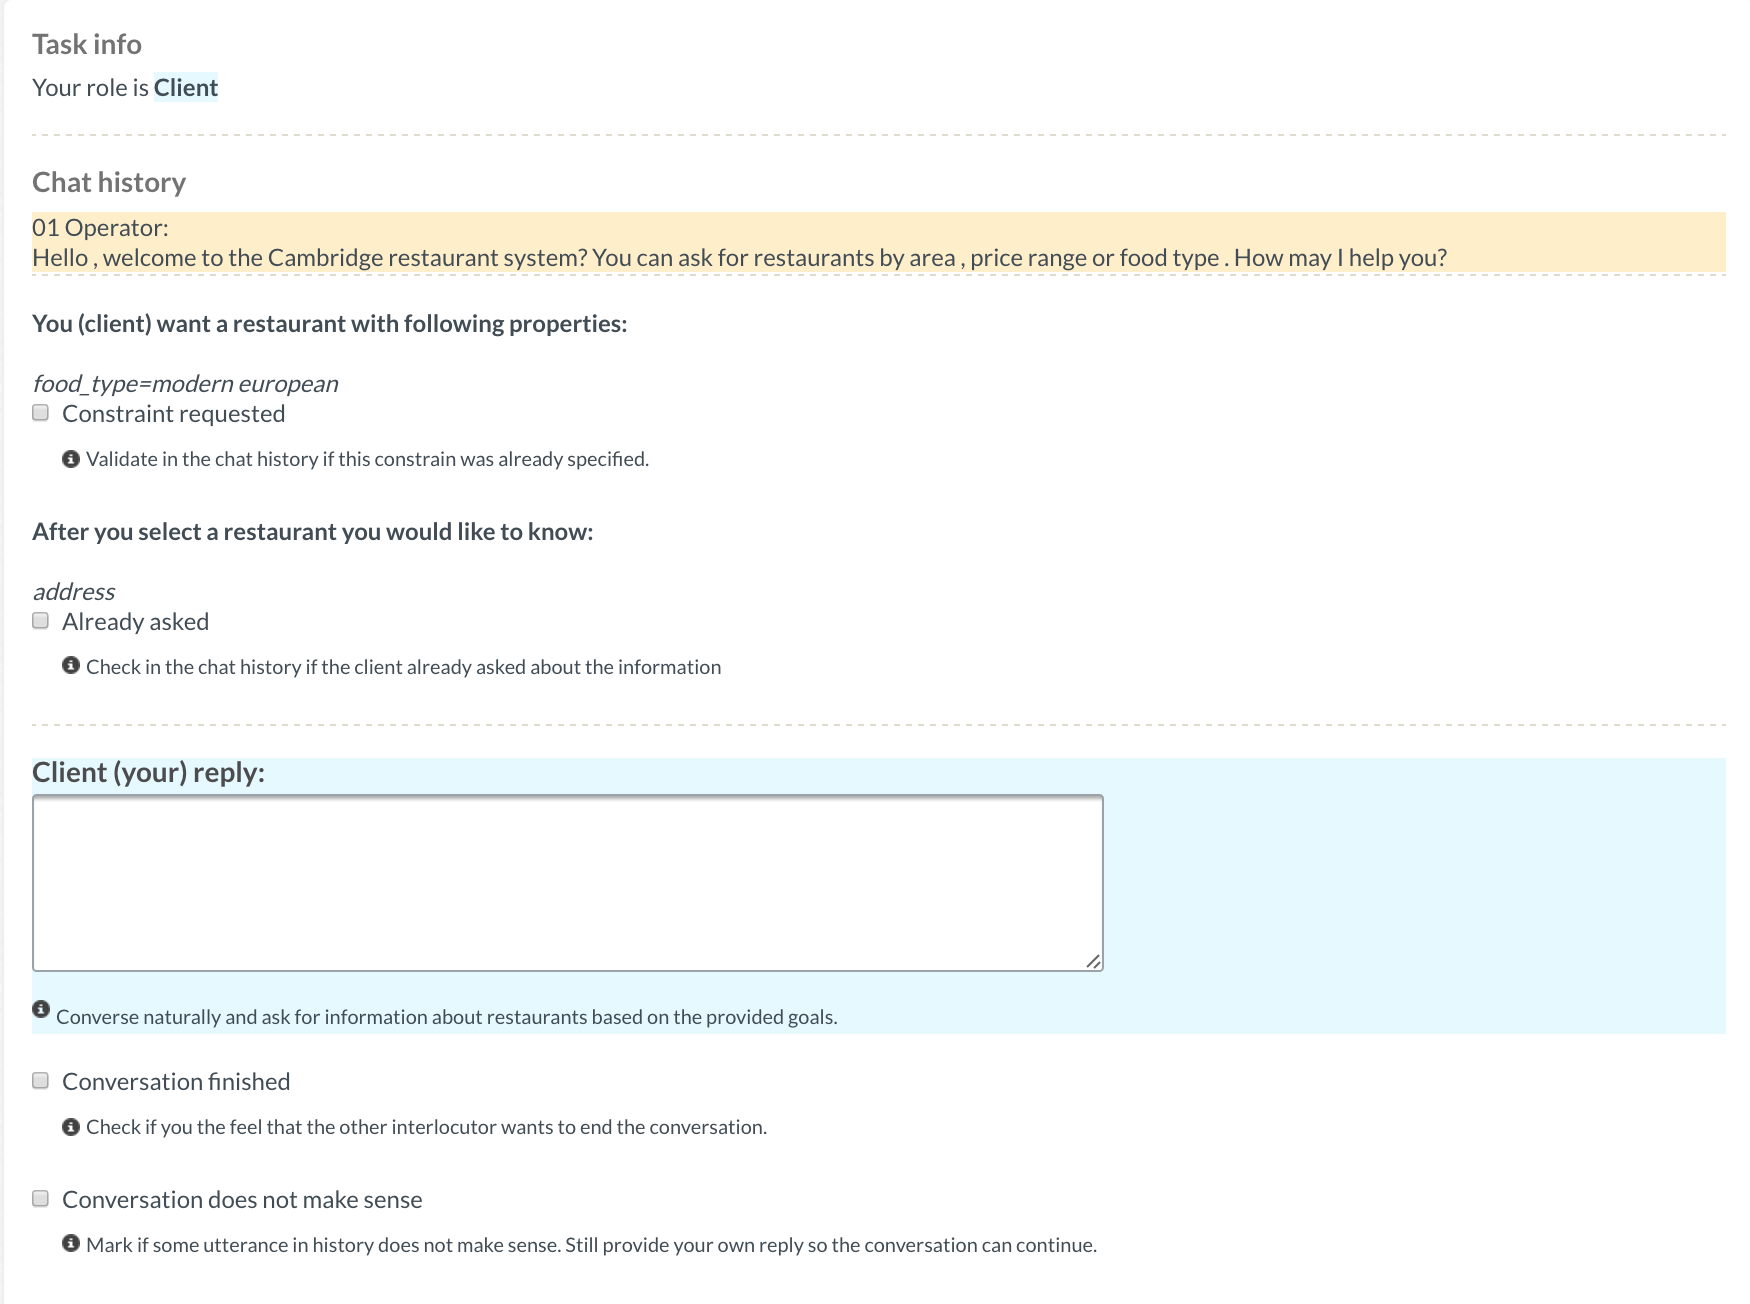
\includegraphics[height=25em]{gui-annotators-client}
\caption{Annotation interface}
\end{center}
\vspace{-0.80em}
\label{fig:encind}
\end{figure}

\section{Dataset Properties}
\label{sec:props}

\begin{table}
\begin{center}
\begin{tabular}{lrr}
\hline
Set   & \# Dialogues & \# Turns \\
\hline
% Joint  &  todo &  todo \\
% /a/SSD/oplatek/e2end/log/2016-06-08-17-31-38.400-dstc-INDEP_labels-d0.7-w100-e100/
% /a/SSD/oplatek/e2end/log/TEST-ORIGINAL-2016-06-08-17-31-38.400dstc-INDEP_labels-d0.7-w100-e100-reward-0.9080-step-0036224
Train  &   ? & ? \\
Dev &   ? & ? \\
Test &   ? & ? \\
\hline
\end{tabular}
\caption{Accuracy on development and test set}
\vspace{-2em}
\end{center}
\label{tab:props}
\end{table}


\section{Related Work}
\label{sec:related}



\section{Conclusion and Future work}
\label{sec:conc}

\subsubsection*{Acknowledgments}
We would like to thank Ond\v{r}ej Du\v{s}ek for useful comments.
This research was partly funded by the Ministry of Education, Youth and Sports of the Czech Republic under the grant agreement LK11221, core research funding, grant GAUK 1915/2015, and also partially supported by SVV project number 260 333. 
We gratefully acknowledge the support of NVIDIA Corporation with the donation of the Tesla K40c GPU used for this research.
Cloud computational resources were provided by the MetaCentrum under the program LM2010005 and the CERIT-SC under the program Centre CERIT Scientific Cloud, part of the Operational Program Research and Development for Innovations, Reg.\ no. CZ.1.05/3.2.00/08.0144.

% ``something in quotes'' using plain tex or use \enquote{the enquote command}.
% cref Demonstration: Cref at beginning of sentence, cref in all other cases.
%
% \Cref{fig:simple} shows a simple fact, although \cref{fig:simple} could also show something else.
%
% \Cref{tab:simple} shows a simple fact, although \cref{tab:simple} could also show something else.
%
% \Cref{sec:intro} shows a simple fact, although \cref{sec:intro} could also show something else.
%
% Brackets work as designed:
% <test>
%
% The symbol for powerset is now correct: $\powerset$ and not a Weierstrass p ($\wp$).
%
% \begin{inparaenum}
% \item All these items...
% \item ...appear in one line
% \item This is enabled by the paralist package.
% \end{inparaenum}
% In the bibliography, use \texttt{\textbackslash textsuperscript} for ``st'', ``nd'', ...:
% E.g., \enquote{The 2\textsuperscript{nd} conference on examples}.
% When you use \href{http://www.jabref.org}{JabRef}, you can use the clean up command to achieve that.


% Winery~\cite{Winery} is graphical \commentontext{modeling}{modeling with one \enquote{l}, because of AE} tool.
%%%%%%%%%%%%%%%%%%%%%%%%%%%%%%%%%%%%%%%%%%%%%%%%%%%%%%%%%%%%%%%%%%%%%%%%%%%%%%%
\bibliographystyle{splncs03}
\bibliography{paper}

All links were last followed on June 28, 2016.
%%%%%%%%%%%%%%%%%%%%%%%%%%%%%%%%%%%%%%%%%%%%%%%%%%%%%%%%%%%%%%%%%%%%%%%%%%%%%%%

\end{document}
